\section{Experiments}
\label{sec:experiments}

\subsection{Experimental Setup}
\label{sec:experimental_setup} 
\textbf{Models.} To demonstrate the effectiveness of \algacro{} and ensure coverage across different model families and sizes, we provide our results on four models: Qwen-2.5-7B~\citep{qwen2024qwen25}, Llama-2-7B~\citep{touvron2023llama}, Llama-3-8B~\citep{dubey2024llama}, and Phi-4-14B~\citep{abdin2024phi}.

\textbf{Data.} We use the Alpaca dataset~\citep{taori2023alpaca} to construct hidden states distribution and compute thresholds for each layer. The Alpaca dataset is an instruction-following dataset for fine-tuning language models, released by a research team from Stanford University with the aim of building and sharing an LLaMA model that follows instructions. The dataset contains 52,000 instructions and demonstrations generated by OpenAI’s text-davinci-003 engine. 

\textbf{Evaluation.}
We use lm-evaluation-harness pipeline~\citep{eval-harness} for our evaluations on an extensive suite of downstream tasks, including PIQA ~\citep{bisk2020piqa},  WinoGrande~\citep{sakaguchi2019winogrande}, HellaSwag~\citep{zellers2019hellaswag}, Arc Challenge~\citep{allenai:arc}, MMLU~\citep{hendrycks2020measuring}, and GSM8K~\citep{cobbe2021training}. 

\textbf{Baselines.} {In practice, the gating strategy can be either top-k-based or threshold-based (\eg, TEAL~\citep{liu2024trainingfreeactivationsparsitylarge} and CATS~\citep{lee2024catscontextuallyawarethresholdingsparsity}). Threshold-based approaches typically determine gating thresholds by statistically analyzing hidden state distributions from a general-purpose dataset. However, directly applying these thresholds during evaluation may cause a mismatch between the actual and target sparsity levels, due to potential distributional shifts between the training and evaluation datasets. To avoid this issue and ensure a fair comparison across methods, we adopt the top-$k$ based gating strategy in our experiments. 

To eliminate the potential effect introduced by the transformation process, we introduce an additional baseline, TEAL-Transform. In this variant, the TEAL approach is applied to the transformed model, retaining the $k$ elements with the largest absolute values $|x|$. This controlled baseline enables a fair comparison of different sparse activation strategies.

To further improve performance, we assign layer-specific sparsity ratios instead of a uniform sparsity across the model. Given a global sparsity target, we leverage the greedy algorithm proposed in TEAL to iteratively configure per-layer sparsity levels such that the aggregate sparsity meets the global budget. This adaptive allocation enables prioritization of computational resources for more critical parameter groups, improving overall performance.


\subsection{Controlled Sparsity Experiments.}
Here, we provide an empirical comparison of \algacro{} against TEAL-based baselines (\eg, TEAL and TEAL-transform) across different sparsity levels (25\% to 65\%) to demonstrate the effectiveness of our proposed algorithm under various experimental settings.

\begin{figure}[t]
    \centering
    \begin{subfigure}[t]{0.24\linewidth}
        \centering
        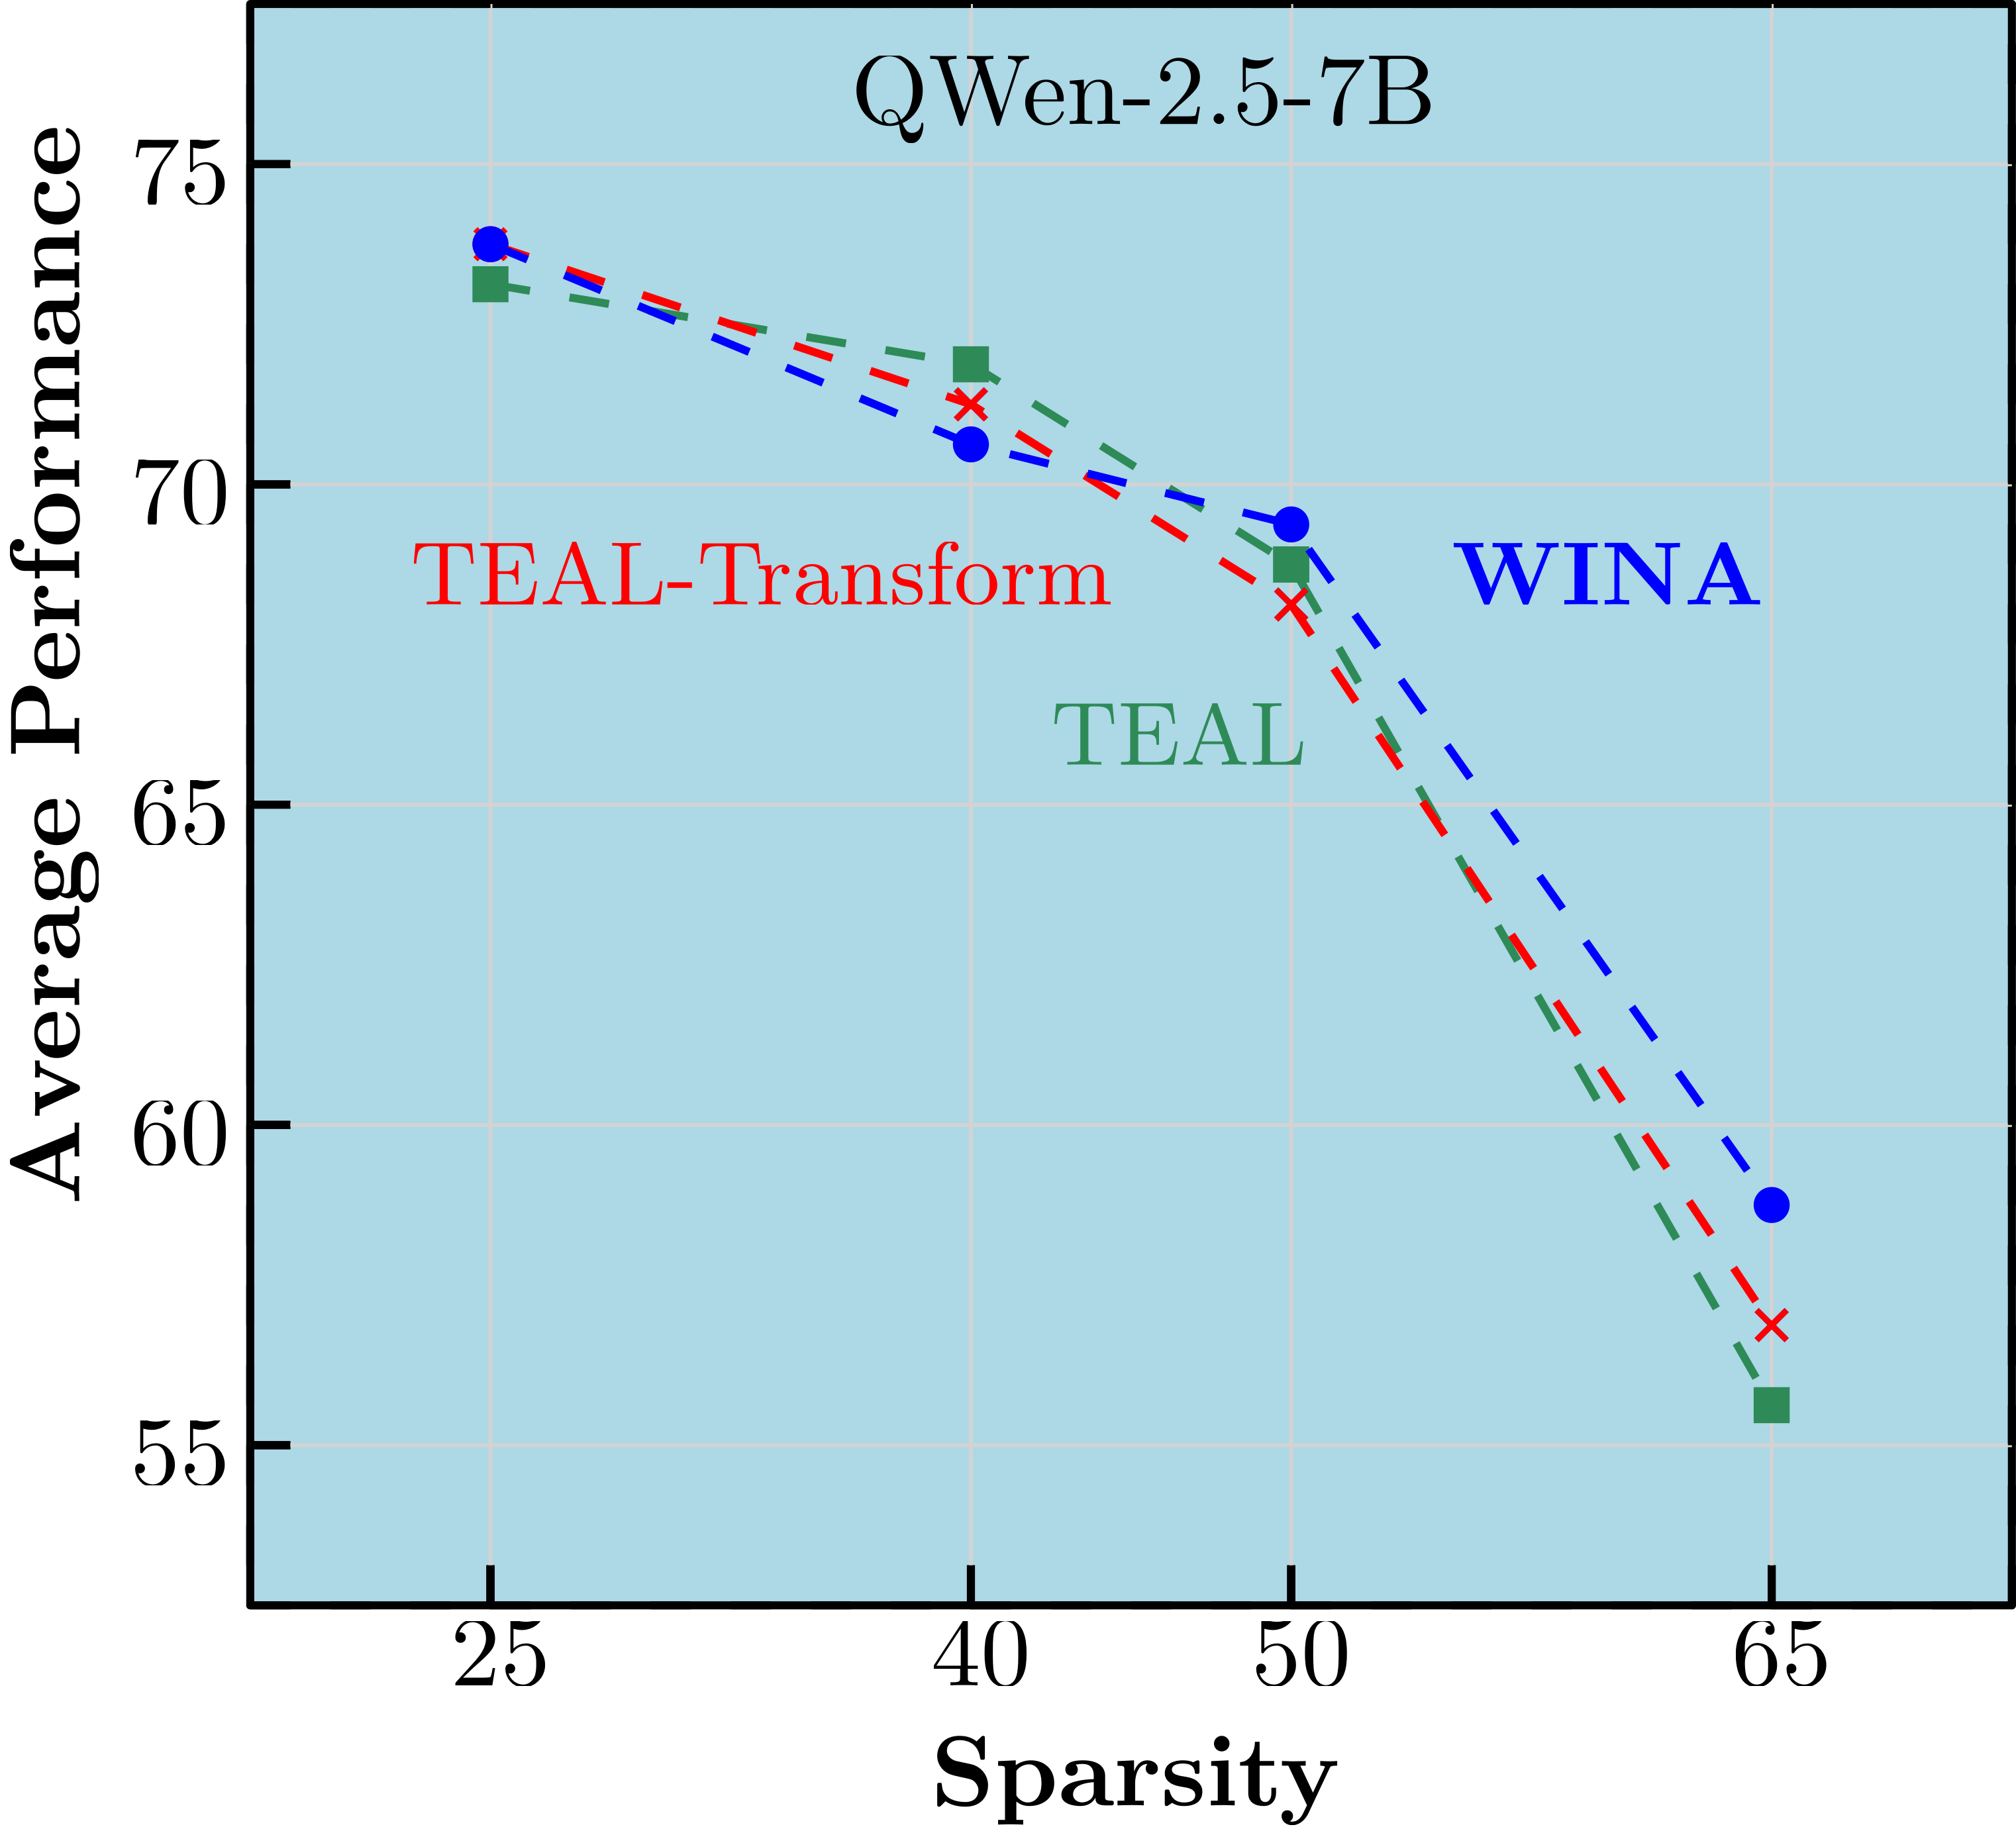
\includegraphics[width=\linewidth]{qwen_2.5_7b.png}
        \caption{QWen-2.5-7B}
        \label{fig:qwen-2.5-7b}
    \end{subfigure}
    \begin{subfigure}[t]{0.24\linewidth}
        \centering        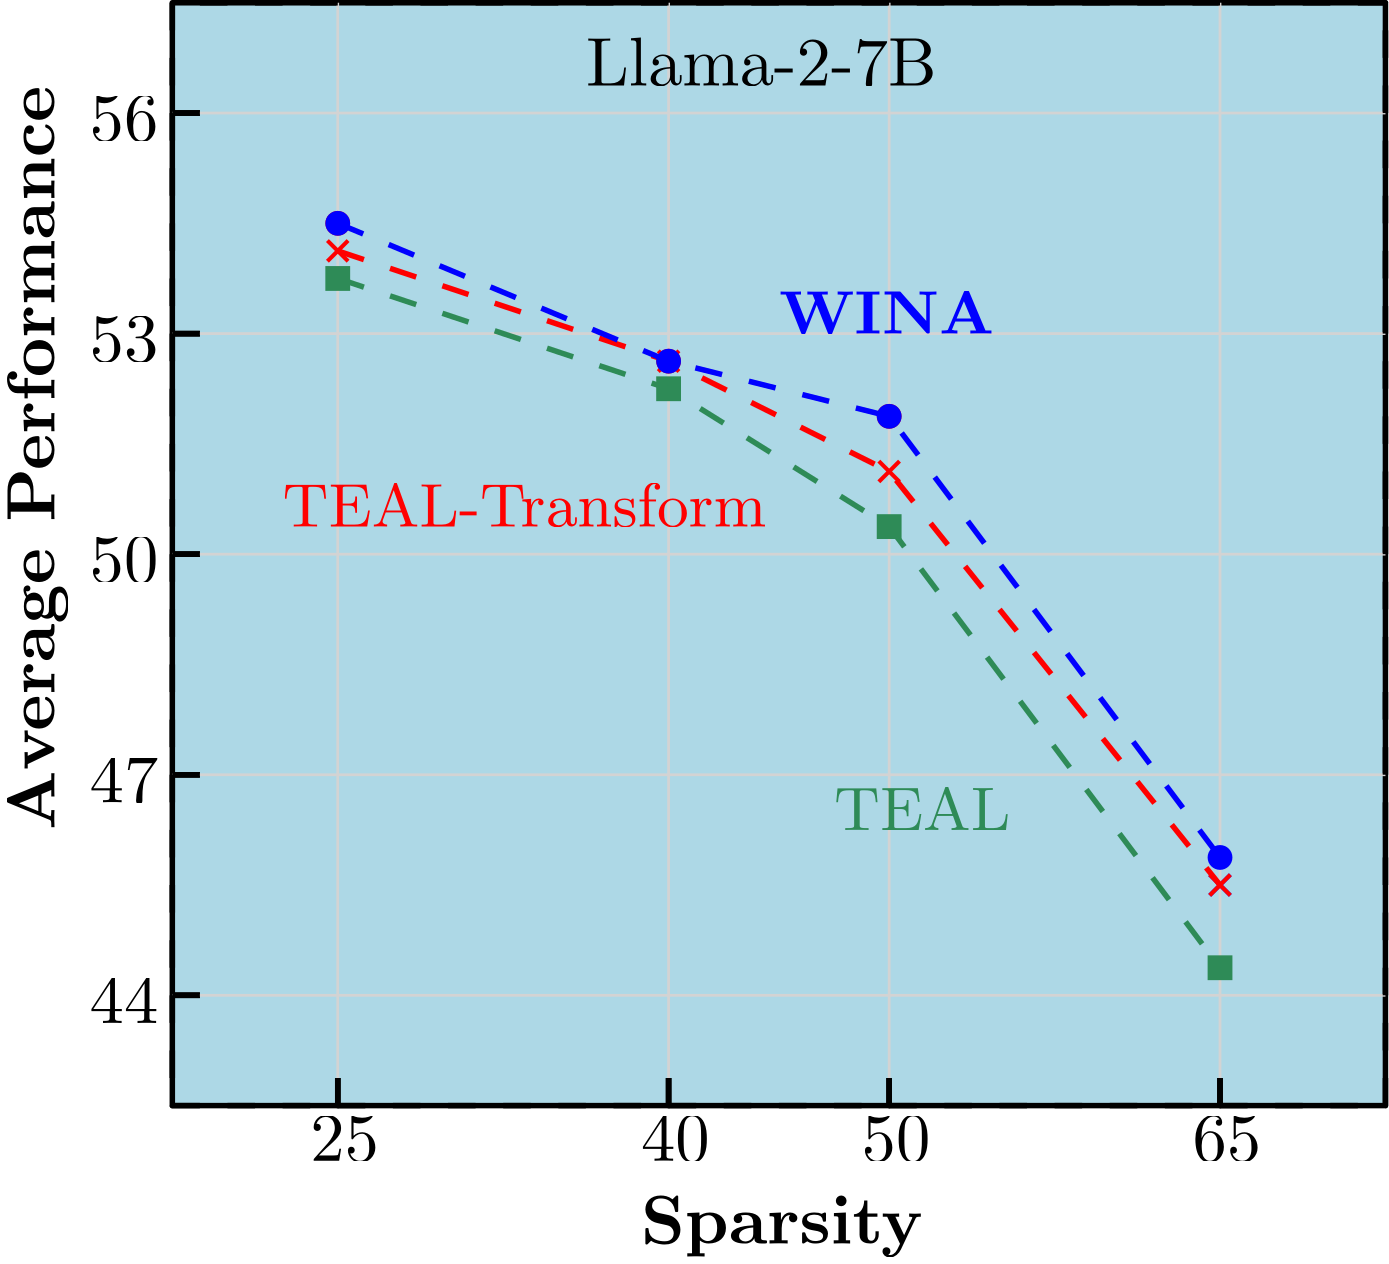
\includegraphics[width=\linewidth]{llama_2_7b.png}
        \caption{Llama-2-7B}
        \label{fig:llama-2-7b}
    \end{subfigure}
    \begin{subfigure}[t]{0.24\linewidth}
        \centering
        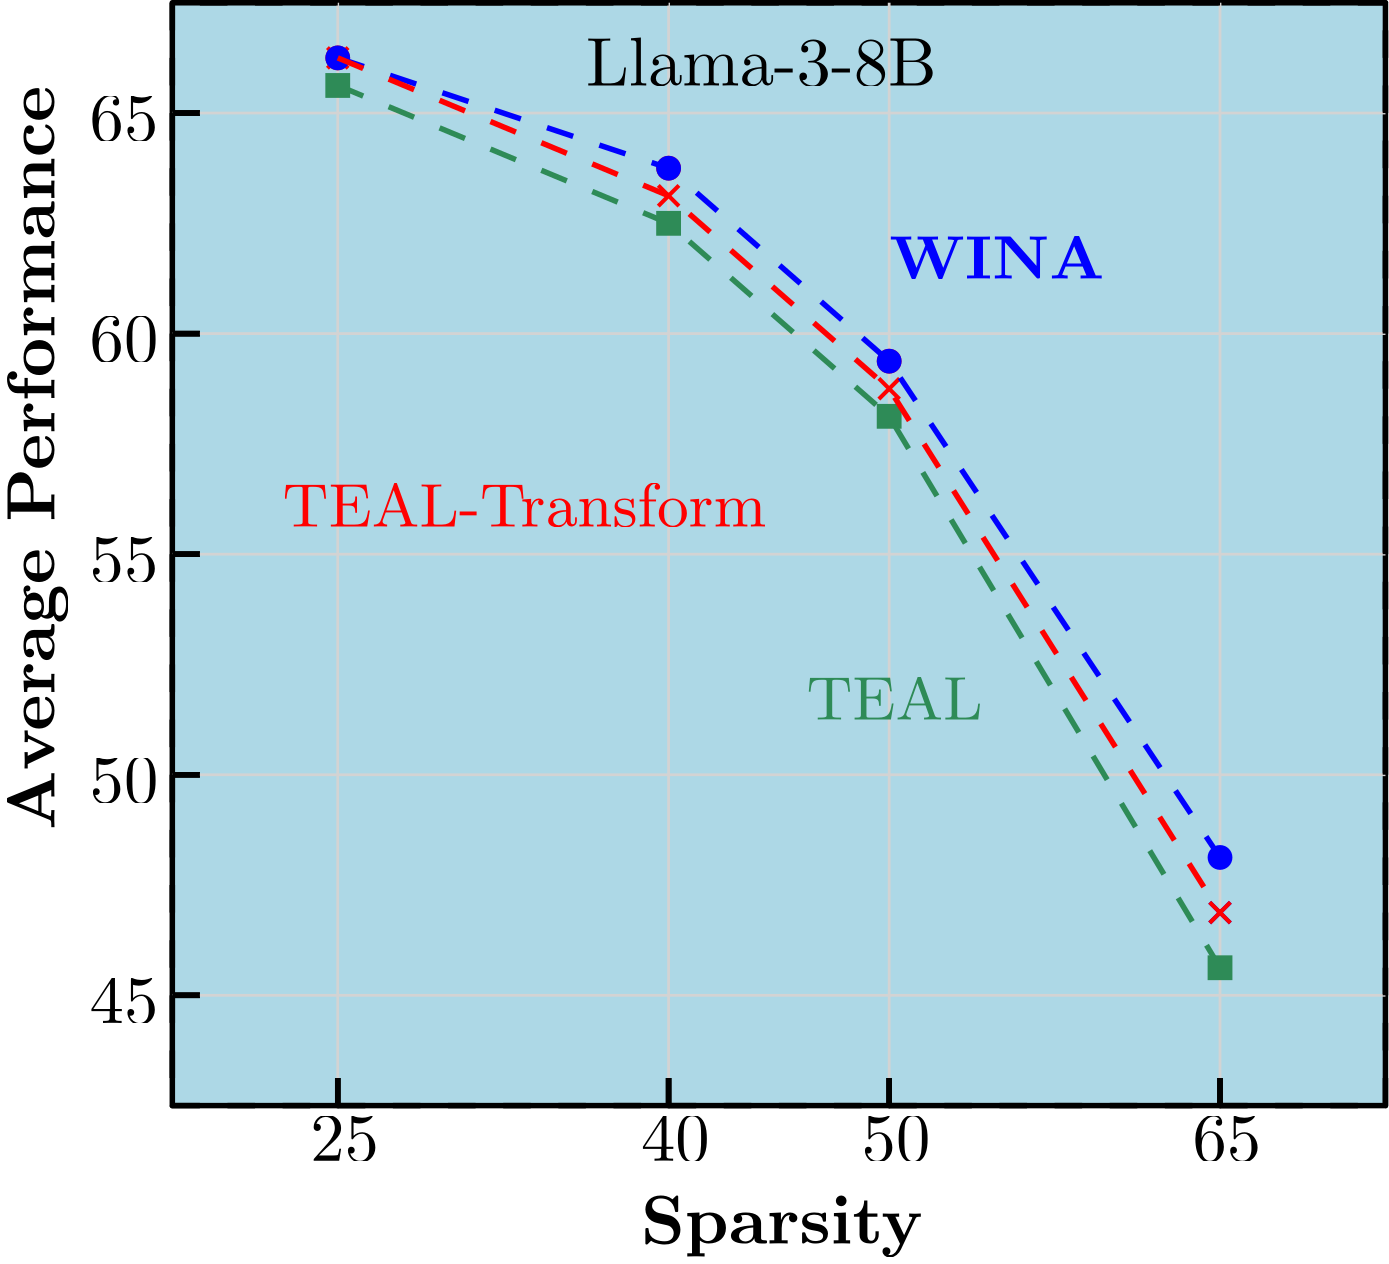
\includegraphics[width=\linewidth]{llama_3_8b.png}
        \caption{Llama-3-8B}
        \label{fig:llama-3-8b}
    \end{subfigure}
    \begin{subfigure}[t]{0.24\linewidth}
        \centering
        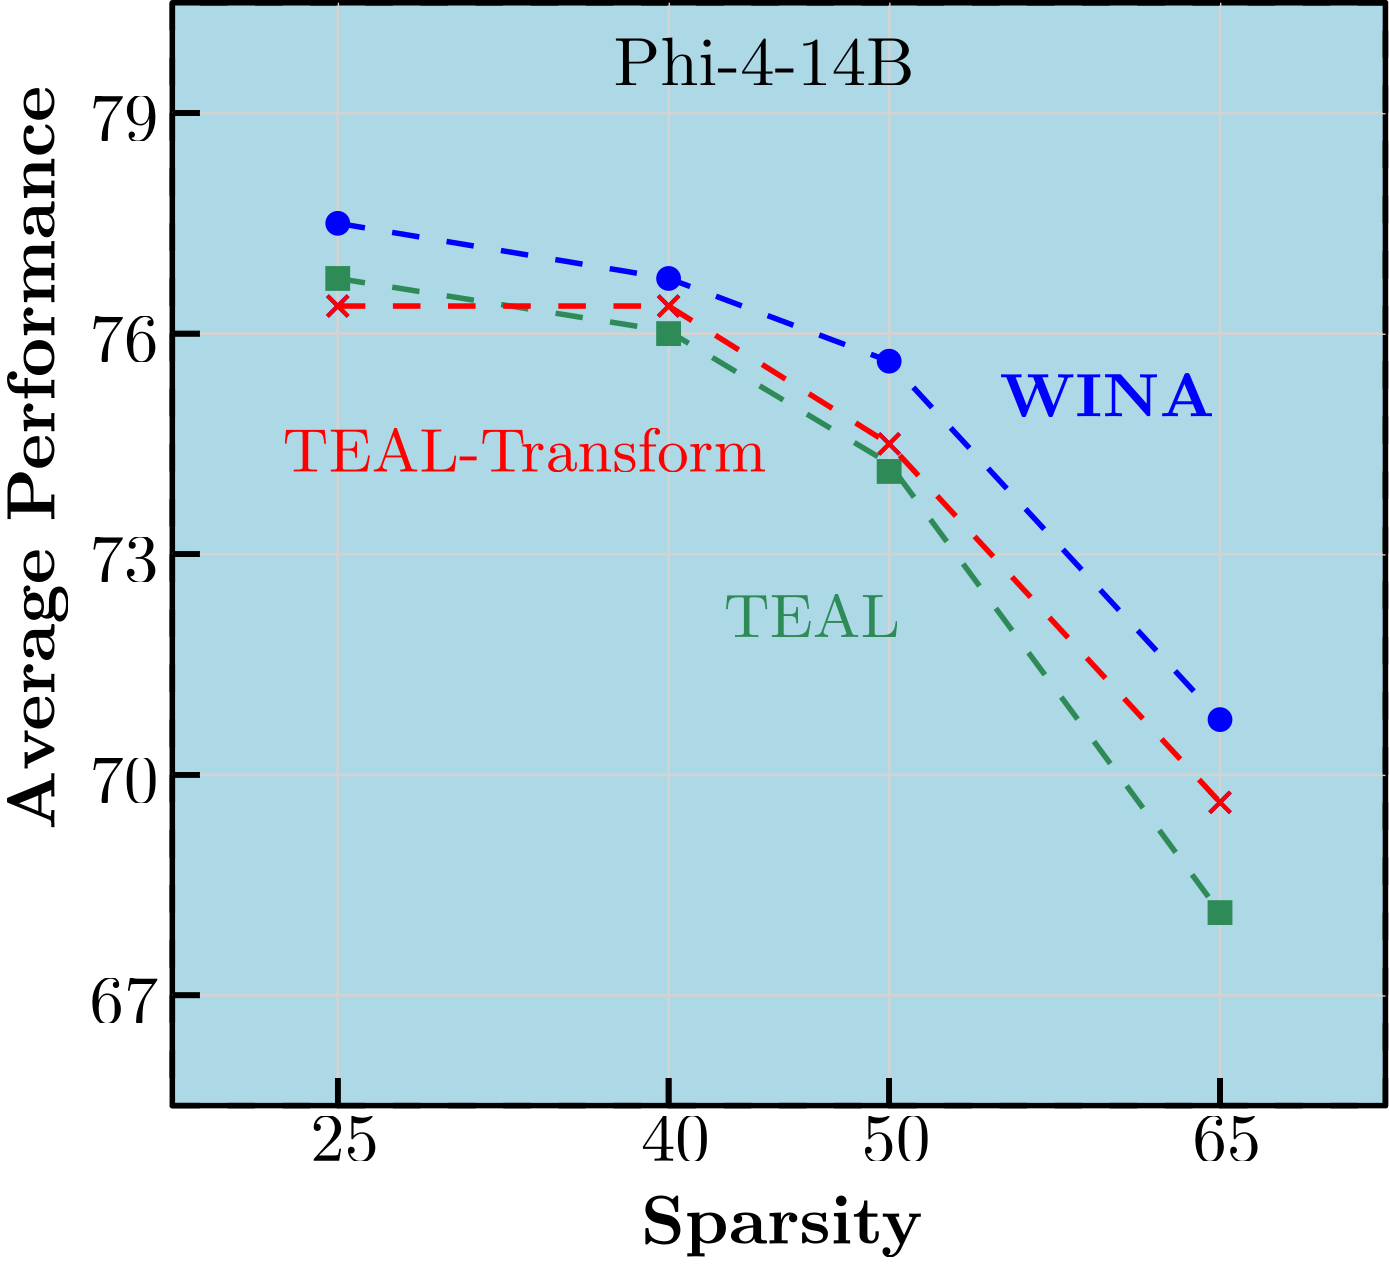
\includegraphics[width=\linewidth]{phi_4_14b.png}
        % \caption{Example caption for Qwen 2.5 7B}
        \caption{Phi-4-14B}
        \label{fig:phi-4-14b}
    \end{subfigure}
    \caption{\textbf{Sparsity-performance frontiers.} Sparsity-performance across Qwen-2.5-7B, Llama-2-7B, Llama-3-8B, and Phi-4-14B.}
    \label{fig:qwen-overview}
\end{figure}

\begin{table*}[t]
  \caption{Results of controlled sparsity experiments over Qwen-2.5-7B}
  \label{tab:qwen25_7b_sparsity}
  \vspace{3pt}
  \centering
  % \addtolength{\tabcolsep}{-1pt}
    \resizebox{1.0\columnwidth}{!}{
\begin{tabular}{llccccccc}
  \toprule[0.1em]
  Method & Sparsity & PiQA & WinoGrande & HellaSwag & Arc-c & MMLU & GSM8K & Avg \\
  \midrule
  Baseline & - & 79.71 & 72.85 & 78.93 & 51.11 & 71.93 & 83.32 & 72.98 \\ \midrule

  \multirow{4}{*}{TEAL~\citep{liu2024trainingfreeactivationsparsitylarge}}  
  & 25\% & 79.27 & 78.56 & 72.77 & 51.19 & 71.30 & 82.87 & {72.83} \\
  & 40\% & 78.40 & 77.28 & 73.09 & 52.65 & 70.20 & 78.32 & \textbf{71.66} \\
  & 50\% & 78.62 & 75.02 & 69.77 & 51.02 & 67.72 & 71.42 & {68.93} \\
  & 65\% & 73.72 & 63.35 & 62.67 & 42.75 & 54.95 & 34.95 & {55.40} \\ \midrule

  \multirow{4}{*}{TEAL-transform} 
  & 25\% & 80.09 & 72.77 & 78.65 & 51.79 & 71.56 & 83.09 & 72.99 \\
  & 40\% & 79.71 & 72.30 & 77.73 & 51.28 & 69.93 & 77.18 & 71.52 \\
  & 50\% & 78.56 & 68.67 & 75.74 & 50.00 & 67.28 & 71.49 & 68.62 \\
  & 65\% & 76.06 & 61.33 & 67.30 & 44.20 & 56.06 & 32.60 & 56.93 \\ \midrule

  \multirow{4}{*}{\algacro{}}  
  & 25\% & 80.05 & 72.69 & 78.58 & 51.37 & 71.51 & 83.93 & \textbf{73.02} \\
  & 40\% & 78.40 & 70.56 & 78.02 & 50.94 & 70.54 & 79.83 & 71.38 \\
  & 50\% & 78.67 & 69.30 & 76.48 & 50.85 & 67.99 & 72.25 & \textbf{69.26} \\
  & 65\% & 76.17 & 61.01 & 70.09 & 42.92 & 59.48 & 38.36 & \textbf{58.34} \\
  \bottomrule[0.1em]
\end{tabular}
  }
\end{table*}

% \begin{table}[t] % [t]表示尽量放在页面顶部
%   \centering
%   \caption{单栏跨栏表格示例}
%   \label{tab:wide}
%   \begin{tabular}{lccr}
%     \toprule
%     Header1 & Header2 & Header3 & Header4 \\
%     \midrule
%     Item1 & 0.25 & 42 & A \\
%     Item2 & 0.67 & 13 & B \\
%     Item3 & 0.92 & 29 & C \\
%     \bottomrule
%   \end{tabular}
% \end{table}
\paragraph{Qwen-2.5-7B.} {We evaluate \algacro{} on Qwen2.5-7B \citep{yang2024qwen2} across various sparsity levels (i.e, 25\% -- 65\%) under the controlled sparsity setting. As shown in \autoref{tab:qwen25_7b_sparsity}, \algacro{} consistently matches or outperforms both TEAL and TEAL -transform across all sparsity levels. Notably, as sparsity increases, the performance gap between \algacro{} and the baselines becomes more pronounced. For instance, at 65\% sparsity, \algacro{} outperforms TEAL by 2.94\% and TEAL-transform by 1.41\% on average. This trend indicates that \algacro{} is more robust under high sparsity, likely due to its ability to retain the most influential activations by jointly considering hidden state magnitudes and weight norms. Particularly on harder tasks such as GSM8K and HellaSwag, \algacro{} maintains relatively strong performance even when aggressive sparsification is applied.}

\begin{table*}[ht]
  \caption{Results of controlled sparsity experiments over Llama-2-7B}
  \vspace{3pt}
  \label{tab:llama2_7b_sparsity}
  \centering
  % \addtolength{\tabcolsep}{-1pt}
    \resizebox{1.0\columnwidth}{!}{
    \begin{tabular}{llccccccc}
  \toprule[0.1em]
  Method & Sparsity & PiQA & Arc-c & WinoGrande & HellaSwag & MMLU & GSM8K & Avg\\
  \midrule
  Baseline & - & 79.05 & 46.33 & 68.98 & 76.00 & 41.82 & 13.87 & 54.34 \\ \midrule

  \multirow{4}{*}{TEAL\,\citep{liu2024trainingfreeactivationsparsitylarge}}  
  & 25\% & 78.18 & 45.99 & 69.85 & 76.01 & 41.30 & 13.34 & 54.11 \\
  & 40\% & 77.53 & 44.45 & 67.88 & 75.32 & 38.66 & 11.07 & 52.49 \\
  & 50\% & 77.53 & 41.21 & 67.25 & 73.57 & 34.71 & 8.79 & 50.51 \\
  & 65\% & 74.43 & 33.87 & 62.12 & 64.20 & 27.05 & 3.56 & 44.21 \\ \midrule

  \multirow{4}{*}{TEAL-transform} 
  & 25\% & 78.45 & 46.42 & 69.14 & 75.93 & 41.75 & 13.42 & 54.19 \\
  & 40\% & 77.69 & 45.48 & 68.43 & 75.18 & 39.22 & 11.05 &  \textbf{52.84} \\
  & 50\% & 78.07 & 43.77 & 66.54 & 73.48 & 36.28 & 10.24 & 51.40 \\
  & 65\% & 74.32 & 37.71 & 63.77 & 66.49 & 29.11 & 3.64 & 45.51 \\ \midrule

  \multirow{4}{*}{\algacro{}}  
  & 25\% & 78.45 & 46.16 & 69.69 & 75.95 & 42.14 & 14.10 & \textbf{54.42} \\
  & 40\% & 77.91 & 45.56 & 67.32 & 75.52 & 39.58 & 11.07 & {52.83} \\
  & 50\% & 78.35 & 44.45 & 67.96 & 73.65 & 36.55 & 9.63 & \textbf{51.76} \\
  & 65\% & 74.59 & 37.88 & 63.93 & 66.55 & 28.81 & 3.18 & \textbf{45.82} \\
  \bottomrule[0.1em]
\end{tabular}
      }
\end{table*}
\paragraph{Llama-2-7B.} {On Llama-2-7B, \algacro{} again shows strong performance under various sparsity constraints. As shown in \autoref{tab:llama2_7b_sparsity}, \algacro{} achieves the highest average accuracy at 25\% sparsity, outperforming both TEAL-based baselines and the full model. While performance naturally degrades at the extreme 65\% sparsity level, \algacro{} still offers the best accuracy, suggesting its robustness under aggressive pruning.}

\begin{table*}
  \caption{Results of controlled sparsity experiments over Llama-3-8B}
  \vspace{3pt}
  \label{tab:llama3_8b_sparsity}
  \centering
  % \addtolength{\tabcolsep}{-1pt}
\resizebox{1.0\columnwidth}{!}{
  \begin{tabular}{llccccccc}
    \toprule[0.1em]
    Method & Sparsity & PiQA & Arc-c & WinoGrande & HellaSwag & MMLU & GSM8K & Avg \\
    \midrule
    Baseline & - & 80.79 & 53.33 & 72.61 & 79.17 & 62.20 & 50.19 & 66.38 \\ \midrule

    % \multirow{4}{*}{TEAL~\citep{liu2024trainingfreeactivationsparsitylarge}}  
    % & 25\% & 80.09 & 53.58 & 72.30 & 78.72 & 61.80 & 50.11 & 66.10 \\
    % & 40\%  & 79.76 & 50.34 & 740\%0 & 77.32 & 59.83 & 42.61 & 63.38 \\
    % & 50\%  & 77.64 & 47.70 & 68.27 & 74.48 & 55.73 & 30.10 & 58.99 \\
    % & 65\% & 72.52 & 37.71 & 60.14 & 58.92 & 33.31 & 3.71  & 44.39 \\ \midrule

\multirow{4}{*}{TEAL~\citep{liu2024trainingfreeactivationsparsitylarge}}  
& 25\% & 80.25 & 53.16 & 73.32 & 78.85 & 61.85 & 48.07 & 65.58 \\
& 40\% & 79.11 & 48.98 & 71.82 & 77.43 & 59.26 & 39.27 & 62.65 \\
& 50\% & 78.24 & 48.12 & 70.01 & 74.83 & 54.50 & 27.37 & 58.51 \\
& 65\% & 73.34 & 37.37 & 63.46 & 61.76 & 32.07 & 4.17 & 45.36 \\ \midrule

    \multirow{4}{*}{TEAL-transform} 
    & 25\% & 80.85 & 53.50 & 73.16 & 78.85 & 61.57 & 47.99 & 65.99 \\
    & 40\%  & 79.43 & 50.60 & 70.88 & 77.36 & 59.23 & 40.11 & 62.94 \\
    & 50\%  & 77.69 & 48.38 & 69.06 & 75.70 & 54.82 & 29.49 & 59.19 \\
    & 65\% & 73.23 & 39.51 & 61.96 & 65.25 & 38.66 & 5.08 & 47.28 \\ \midrule

    \multirow{4}{*}{\algacro{}}  
    & 25\% & 80.79 & 53.16 & 73.24 & 78.96 & 61.54 & 48.29 & \textbf{66.00} \\
    & 40\%  & 79.60 & 50.09 & 71.27 & 77.54 & 58.82 & 41.85 & \textbf{63.20} \\
    & 50\%  & 78.35 & 49.06 & 70.32 & 75.12 & 55.26 & 29.34 & \textbf{59.57} \\
    & 65\% & 73.45 & 40.10 & 62.67 & 64.89 & 38.48 & 7.05 & \textbf{47.77} \\
    \bottomrule[0.1em]
  \end{tabular}
    }
\end{table*}
\paragraph{Llama-3-8B.} The results on Llama-3-8B further emphasize \algacro{}’s resilience to pruning, as summarized in \autoref{tab:llama3_8b_sparsity}. While TEAL slightly outperforms at the 25\% level, \algacro{} leads in all remaining sparsity configurations, culminating in +1.06\% and +2.41\% over TEAL at 50\% sparsity and 65\% sparsity, respectively. Notably, \algacro{} sustains particularly strong performance on reasoning-intensive tasks like GSM8K and ARC Challenge, where other methods show significant drops under compression. These patterns suggest that \algacro{} is not only compression-friendly but also capable of preserving complex decision-making abilities under tight computational budgets.

\begin{table*}
  \caption{Results of controlled sparsity experiments over Phi-4-14B}
  \label{tab:phi4_14b_sparsity}
  \vspace{3pt}
  \centering
  % \addtolength{\tabcolsep}{-1pt}
\resizebox{1.0\columnwidth}{!}{
  \begin{tabular}{llccccccc}
    \toprule[0.1em]
    Method & Sparsity & PiQA & WinoGrande & HellaSwag & Arc-c & MMLU & GSM8K & Avg \\
    \midrule
    Baseline & - & 81.28 & 76.80 & 81.93 & 55.97 & 77.06 & 90.22 & 77.21 \\ \midrule

  \multirow{4}{*}{TEAL~\citep{liu2024trainingfreeactivationsparsitylarge}}  
  & 25\% & 81.07 & 75.45 & 81.92 & 56.23 & 76.63 & 89.84 & 76.86 \\
  & 40\% & 80.79 & 73.80 & 81.21 & 54.95 & 75.10 & 88.02 & 75.98 \\
  & 50\% & 80.63 & 71.98 & 80.06 & 53.84 & 73.52 & 86.13 & 74.36 \\
  & 65\% & 77.64 & 66.06 & 74.26 & 50.77 & 65.17 & 74.37 & 68.71 \\
  \midrule

  \multirow{4}{*}{TEAL-transform} 
  & 25\% & 80.96 & 74.59 & 81.60 & 55.63 & 76.68 & 89.92 & 76.56 \\
  & 40\% & 81.18 & 74.19 & 80.94 & 54.61 & 75.99 & 90.07 & 76.50 \\
  & 50\% & 79.82 & 72.38 & 79.79 & 53.92 & 74.51 & 88.02 & 74.74 \\
  & 65\% & 77.64 & 68.51 & 74.72 & 52.47 & 66.64 & 77.18 & 69.86 \\
  \midrule

\multirow{4}{*}{\algacro{}}  
& 25\% & 81.01 & 75.37 & 81.91 & 56.31 & 76.60 & 90.22 & \textbf{77.57} \\
& 40\% & 81.18 & 72.45 & 81.44 & 56.06 & 76.44 & 90.67 & \textbf{76.71} \\
& 50\% & 81.39 & 73.95 & 81.75 & 54.95 & 75.83 & 87.57 & \textbf{75.91} \\
& 65\% & 78.24 & 70.72 & 77.10 & 51.11 & 70.05 & 77.10 & \textbf{70.72} \\
    \bottomrule[0.1em]
  \end{tabular}
  }
\end{table*}


\paragraph{Phi-4-14B.} \algacro{} also delivers robust performance on Phi-4-14B across all tested sparsity levels, as detailed in \autoref{tab:phi4_14b_sparsity}. It consistently either matches or exceeds the accuracy of both TEAL and TEAL-transform, and achieves the top average score at every sparsity setting. At the highest sparsity of 65\%, for instance, \algacro{} improves upon TEAL and TEAL-transform by +2.01\% and +0.86\%, respectively. Its ability to retain high performance on complex benchmarks such as GSM8K and MMLU, even under severe pruning, highlights its stability. These outcomes demonstrate that \algacro{} can effectively preserve key reasoning mechanisms in large-scale models, making it well-suited for sparsity-constrained deployments.

\begin{table}[H]
\centering
\caption{(G)FLOPs over different sparsity across diffrent model architecture.}\label{tab:gflops}
\begin{tabular}{lcccc}
\toprule
Sparsity & QWen2.5-7B & Llama-2-7B & Llama-3-8B & Phi-4\\
\midrule
Baseline & 7.07 & 6.61 & 7.50 & 14.15  \\
\midrule
0.25 & 5.44 ($\downarrow 23.1\%$) & 4.99 ($\downarrow 24.5\%$) & 5.76 ($\downarrow 23.2\%$) & 10.74($\downarrow 24.1\%$)\\
0.4 &  4.46 ($\downarrow36.9\%$) & 4.02 ($\downarrow39.2\%$) & 4.71 ($\downarrow37.2\%$) & 8.69 ($\downarrow38.6\%$)\\
0.5 & 3.81 ($\downarrow46.1\%$) & 3.37 ($\downarrow49.0\%$) & 4.01 ($\downarrow46.5\%$) & 7.33 ($\downarrow48.2\%$)\\
0.65 & 2.83 ($\downarrow60.0\%$) & 2.40 ($\downarrow63.7\%$) & 2.97 ($\downarrow60.4\%$) & 5.28 ($\downarrow62.7\%$)\\
% \midrule
% {\algacro{} Avg Acc.} & 73.02 & 54.42 & 66.00 & 77.57 \\
\bottomrule
\end{tabular}
\end{table}
\paragraph{Acceleration.} In addition to performance gains, \algacro{} yields substantial computational acceleration across all evaluated LLMs. As shown in~\autoref{tab:gflops}, \algacro{} reduces the overall (G)FLOPs by up to 60.0\% on Qwen-2.5-7B, 63.7\% on Llama-2-7B, 60.4\% on Llama-3-8B, and 62.7\% on Phi-4-14B at the 65\% sparsity level. These consistent reductions in floating point operations could translate to faster inference speeds and lower computational costs, validating \algacro{}’s effectiveness as a practical solution for deployment under tight resource constraints. 
% Notably, these accelerations are achieved without requiring any model retraining, highlighting the plug-and-play nature of our training-free framework.





% \input{src/tab_llama2_13b}
% all results are buged.
% \input{src/tab_mistral_7b}



% \subsection{Empirical Sparsity Analysis.}